\chapter{Physical Implementation}

// TODO: add diagram of physical components and their connections
This chapter describes our choosing of physical components, and the implementation of the \gls{pcb}.

\section{Architecture}
The main specification the group had to meet at all costs was to be able to take a program (a sequence of instructions) as input, and output vector graphics on a screen.

Tracing the envisioned execution path of a program through the system gives insight into some of the considerations that had to be taken when designing the \gls{pcb} and selecting components. An overview of the \gls{pcb} architecture is displayed in \ref{fig:PCB_Overview}

\begin{enumerate}
\item Assembled \vthreek programs are loaded into instruction memory via the EFM32 microcontroller.
\item The \gls{fpga} reads instructions from memory and performs execution.
\item Data ready to be sent to output will be stored in a frame buffer.
\item The \gls{fpga} sends data from the frame buffer to the output screens via two interfaces, two \gls{dac}s and an \gls{hdmi} port.
\item The output from the \gls{dac}s is displayed on an analogue oscilloscope and the output from the \gls{hdmi} on a raster screen.
\end{enumerate}

The plan with the flash memory was to be able to store the bit file, which would configure the \gls{fpga}. This would make us able to quickly get the system up and running after turning it on, since the flash would automatically be configured.

\begin{figure}[h!]
\centering
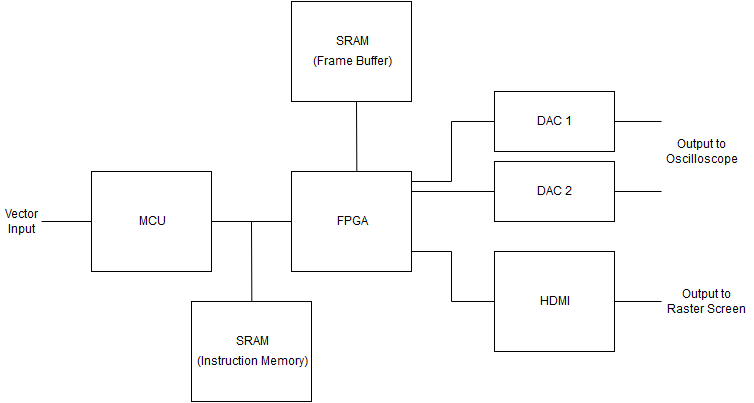
\includegraphics[scale = 0.4]{images/PCB_Overview.png}
\caption{Overview of \gls{pcb} architecture}
\label{fig:PCB_Overview}
\end{figure}

\section{Components}
This section describes the team's choices of components.
All components had to meet the team's technical demands, e.g. number of pins, voltage level support and satisfying outputs.
This information was found by inspecting the various component's datasheets.
Critical components in the design are described in the following subsections.

\subsection{MCU}
The \gls{mcu} was the EFM32GG microcontroller described earlier. 

\subsection{FPGA}
The \gls{fpga} was a Xilinx XC6SLX45-2CSG324I, with 401 kb block \gls{ram}. 
It served as the main processor in the design, fetching and executing instructions from instruction memory.

A \gls{jtag} header was connected to the \gls{fpga} for good accessibility to \gls{fpga} debugging and programming.
//TODO : elaborate

\subsection{SRAM}
Two \gls{sram}s were put on the \gls{pcb}. 
One of them worked as an instruction memory for the \gls{fpga}, while the other was a dedicated frame buffer for our output signals. 
The instructions executed in the \gls{fpga} would update the frame buffer, and data from the frame buffer could be read and transferred to the output units. 
Both \gls{sram}s had an address space of 512k 16-bit words. 

\subsection{DACs and BNCs}
As the purpose of the computer was to output vector graphics on an analogue vector screen, \gls{dac}s were essential.
They would convert digital signals from the \gls{fpga} destined for the output screen, to corresponding analogue signals.

It was important that the \gls{dac}s could output signals fast enough, to minimize flickering. 
Therefore, \gls{dac}s that could support clock rates up to 30MHz was chosen.

The \gls{bnc}s connectors would receive the analogue signals and send them to the oscilloscope.
There was one \gls{dac} and one \gls{bnc} for both the x-coordinate and the y-coordinate on the oscilloscope.

\subsection{Oscillators}
Two external oscillators were connected to the \gls{mcu}: one low frequency (32,768kHz), and one high frequency (48MHz).
The \gls{mcu} already contained internal RC-oscillators, but external oscillators were much more accurate and stable than the internal ones, which was important for avoiding more sources of errors.
Both crystals or full-fledged oscillators could be used, but in the end, the team decided to use oscillators.
The reason behind this choice was that an oscillator was one fully built component with all the necessary circuitry inside, and the datasheet clearly specified how it should be connected.
Crystals, on the other hand, required load capacitors, whose values weren't properly specified.
Another reason was that our \gls{fpga} explicitly needed an external oscillator, as a crystal was incompatible with the design.
Hence, the team chose oscillators for both the \gls{fpga} and \gls{mcu} for simplicity.

\subsection{Buses}
The system used one parallel bus (\gls{ebi}), and one serial bus (\gls{spi}).
The \gls{mcu} acted as bus master for both of them, since it supplied the bus technologies.

\subsubsection{EBI}
The \gls{fpga}, \gls{mcu} and \gls{sram} were all connected via the \gls{ebi} bus.
These connections were made properly by using the specified \gls{ebi}-pins on the \gls{cmu}. // TODO: citation to \gls{mcu} datasheet
The \gls{ebi} bus allowed high-speed communication to the \gls{sram}.
As the \gls{ebi} bus is a parallel bus, the team included the following bus lines:
\begin{itemize}
\item 23 Address bits. More than initially needed, but this was increased for good measure.
\item 16 Data bits, since our \gls{sram} consisted of 16-bit words.
\item 2 Chip select bits, one for the \gls{fpga} and one for the \gls{sram}.
\item 1 Write enable bit, active low.
\item 1 Read enable bit, active low.
\end{itemize}

\subsubsection{SPI}
The \gls{spi} served as a three-way communication between the \gls{mcu}, \gls{fpga} and Flash memory.
It's main purpose was to make the \gls{fpga} be configured from a bit-file stored in the flash memory.
As opposed to the \gls{ebi} bus, \gls{spi} is a serial bus, transferring one bit of data at a time.

\subsection{Buttons and LEDS}
All buttons included a resistor for current limitation (to avoid short circuits) and pull-up (to avoid logical floating state).
The exception was the button connected to the \gls{mcu}, where the pin had an internal pull-up.
All \gls{led}s also included a current limiting resistor. 
Ohms law was used to calculate the required resistance\cite{ohm}.

\gls{led}s were handy for giving an indication that something was turned on. 
For instance, the design included a \gls{led} which would light up when the \gls{fpga} was configured.
Buttons were used for triggering events, e.g. reset.

\subsection{Power Supply}
The \gls{pcb} would receive power from a micro-\gls{usb} connector. 
A voltage level of 5V was sufficient, since no components required more than this. 
However, plenty of components required less than 5V, specifically 3.3V. 
To lower the voltage to a specific level, voltage regulators were used. 
Power is discussed in more detail in section \ref{Power}.

\subsection{Decoupling Capacitors}
Several major components required decoupling, e.g. the \gls{mcu}, \gls{fpga}, voltage regulators and \gls{dac}s.
Decoupling means connecting power supplies through a capacitor network to ground, where power moving to ground can be temporarily stored.
This is necessary as it sometimes occurs situations where there is suddenly high need for power.
The power supply alone would not always be able to support these 'bursts'.
With a capacitor decoupling network, the component could pull power from the capacitors instead.

\section{PCB Design}
The architecture was realized on a \gls{pcb} designed using Altium Designer 15.1.
Having never used this program before, the group had to overcome challenges and difficulties related to not only learning new software, but also learning concepts of creating a \gls{pcb} from scratch. 

\subsection{Schematics}
The entire logic on the \gls{pcb} was designed with schematics. 
Altium was used to map the components together, pin by pin. 
Making the right connections and pin mappings was the only thing that mattered in the schematics. 
There was no focus on physical \gls{pcb}-specific things, e.g. routing and component placement.

When the schematics were completed, the team moved on to design the physical \gls{pcb}.

\subsection{Component Placement}
The goal was to place the components on the \gls{pcb}, so that they preferably were in close range of all other components they had to connect with. 
This would shorten the routing, which was desirable in terms of mitigating signal delay and maintaining signal integrity.

The \gls{fpga}, \gls{sram}s and \gls{mcu} were the most important components with a lot of different connections, and were therefore placed central on the \gls{pcb}.
\gls{io} components, e.g. controller buttons, \gls{usb}, \gls{hdmi} and \gls{bnc} receptacles, were placed along the edge, since these were typically connected to few other components.
It would also be annoying to connect external peripheral plugs to sockets in the middle of the \gls{pcb}.

All decoupling capacitors involved in the decoupling network for a certain component, were placed in close proximity to that component.
This minimized the risk of that the component wouldn't get the extra power supply it needed during bursts.
All capacitors and resistors were placed on the bottom layer of the \gls{pcb} to save space on an already crowded top layer.

\subsubsection{Component Footprints}
A component footprint is how the trace of a component looks like on the \gls{pcb}.
In the beginning, component footprints from the standard Altium library were used.
After previewing the board, it became clear that these footprints were in fact gigantic, and footprints of suitable size had to be found using Altium vaults.
Smaller 0603 (1608 metric) footprints were used for most passive components, especially the capacitors and resistors.
By standardizing footprint sizes, the bill of materials could easily be updated without changing the \gls{pcb} design, as long as the new component could be found in the same package size.
While a trade-off by using this small size package is that the components might be trickier to solder onto the board, the gain in size reduction for the board as a whole were valued higher by the group.
Some components could not be found in this footprint, but luckily there was no shortage of footprint sizes to choose from.

\subsection{Layers}
The \gls{pcb} consisted of six signal layers: Top layer, bottom layer and four in between.
Two power layers were utilized: \(V_{CC}\) and ground.
Between every signal and power layer, a dielectric layer was added to ensure proper isolation between these conducting layers, such that they wouldn't interfere with each other.

An overlay was added to both the top and bottom layers.
The overlay was added to contain silk-screen for marking components, thus making it easier to navigate the \gls{pcb}.

The complete layer stack is shown in figure \ref{fig:Layers}

\begin{figure}[h!]
\centering
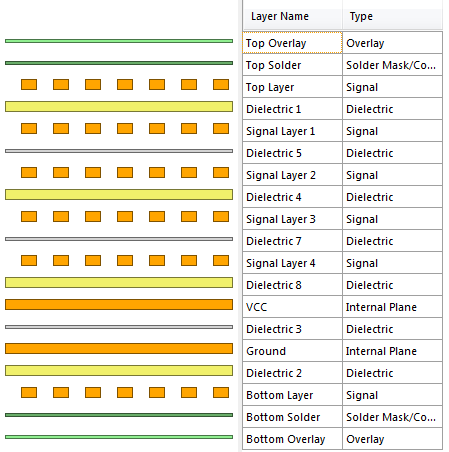
\includegraphics[scale = 0.8]{images/Layers.png}
\caption{Layer Stack}
\label{fig:Layers}
\end{figure}

\subsubsection{Power and ground}
\label{Power}
The \gls{pcb} was designed with three power domains, each with their corresponding voltage regulator: 3.3V, 1.2V and a 5V reserved for analogue signals.
Most components were supplied by the 3.3V regulator, except for some internal parts of the \gls{fpga} that required 1.2V.

Since 3.3V was used by most components, and since only a few connectors required 1.2V, a dedicated power plane for 3.3V was added.
A dedicated ground plane was also added.
This prevented more unnecessary routing, since everything connected to 3.3V or ground could go straight to a via by dogboning, and automatically be connected to the corresponding plane. 
The 1.2V traces had to be routed through all the connectors like any other signal. 

\subsubsection{Split planes}
The story of analogue 5V is a little different. 
The reason for an analogue 5V was to avoid noise from digital signals. 
The analogue components are sensitive to noise from the digital circuitry, and it was crucial to have as little noise as possible on the signal going to the oscilloscope. 
To avoid noise, the analogue and digital circuitry had to be separated completely. 
Analogue components could not use the same voltage supply as the digital ones, and the same mattered for ground.

The solution was to split the power and ground plane, shown in figure \ref{fig:Split planes}. 
\begin{itemize}
\item 5AV: Analogue 5V for components on the analogue plane. 
The reason for 5V was based on insecurity about how much voltage the oscilloscope required to properly display the vector graphics from the program. 
3.3V could be too low, so 5V was chosen. 
A high signal voltage could also potentially help reduce noise.
\item AGND: Analogue components are connected to this ground instead of digital ground. 
This is to stop the analogue signal from getting disturbed by the digital signals on the ground plane.
\item 3.3V: Digital voltage for digital components.
\item GND: Digital ground.
\end{itemize}

All analogue components were placed in the analogue plane, and the opposite with digital components. 
The exception was the \gls{dac}s, which acts as a bridge between the digital part and the analogue part. 
These were placed on the actual split, with the affected pins on the correct side.

To remove any digital noise that could potentially accumulate on the analog ground plane, a diode was placed between the two ground planes. 
This let the current flow from the analogue ground to the digital ground, but not vice versa.

\begin{figure}[h!]
\centering
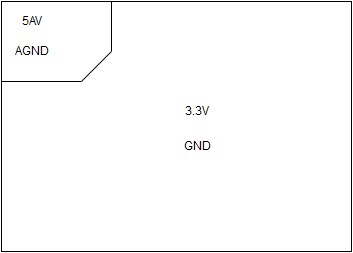
\includegraphics[scale = 0.6]{images/Split_planes.png}
\caption{Split between analogue and digital planes. The separating line is a solid, non-conducting material}
\label{fig:Split planes}
\end{figure}

\section{Routing}
The components had to be physically connected according to the schematics.
Connections could be manually routed, or Altium's auto router could be used. 
The auto router would automatically route as many connections as possible.  

Routing was a much more time-consuming process than the team expected. 
Too much trust was put into Altium's auto router. 
The router did not, as the team naively thought, magically solve the routing. 

\subsection{Design Rules}
Before routing, necessary rules had to be defined to make sure the \gls{pcb} was routed properly. 
The following listing explains the most important rules for the design.
\begin{itemize}
\item Clearance: 0.1mm. 
\newline
Minimum clearance between different traces
\item Width: 0.127mm, Power Width 0.203mm.
\newline
Minimum width for traces. 
Power traces had bigger minimum widths, than signal traces.
\item Via Diameter: 0.4mm, Via Hole Size: 0.2mm
\newline
Minimum diameter and hole size for multi-layer vias.
\item Short-circuits and net antennas not allowed
\end{itemize}

The rules were set like this to make sure there wouldn't be any interference between traces, while the traces were still wide enough to not be damaged by the signal itself. 
Power traces were wider to make sure they could handle the voltage.
Net antennas were traces that lead to dead-ends. 
This could harm the design, since these dead-ends could work as unwanted signal receivers from nearby sources.

\subsubsection{Design Rule Check}
Altium had it's own tool for testing how many violations our current design created, called Design Rule Check. 
It displayed the amount of errors occurred from each type, and the coordinates on the \gls{pcb} for every error. 
Typical errors during our design procedure were short-circuits, net antennas and clearance constraint violations.

\subsection{Routing Procedure}
The task of routing the \gls{pcb} was started by routing some components manually. 
The team quickly discovered that doing this for the entire board would take a very long time, and so began to check out Altium's built-in auto router. 
//TODO: Add source

The team ran into many different routing problems, which is discussed in detail in section \ref{Routing Problems}

\section{Fault Handling}
The team were all inexperienced with \gls{pcb} design and often uncertain if actions or decisions could cause problems down the line. 
The top priority was to make something that worked properly. 
A failing component was deemed probable, and forgetting something was guaranteed to happen, considering the vast amount of factors involved. 
Hence, the team decided that having back-up features on the \gls{pcb} was critical.

\subsection{Headers}
The primary strategy of handling faults was redundancy, mostly in the form of header pins. 
The final amount of headers ended up at 34, including the \gls{jtag} and the ARM programming header. 
Using this huge amount of headers made it possible to measure most signals with a multimeter and verify them. 
The team got this idea from reading the Demolicious report \cite{demolicious-report}, from last years computer design project. 

Most headers were placed between components. 
If wrong connections existed, or a connection didn't work, the connection could hopefully be corrected by connecting wires. 
Not only could errors more easily be detected - it would also be easier to fix them.

\begin{figure}[h!]
\centering
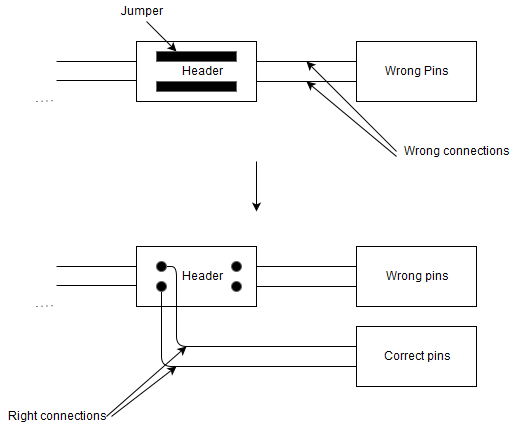
\includegraphics[scale = 0.45]{images/Header_fix.png}
\caption{Example Header fix}
\label{fig:Header fix}
\end{figure}

Headers was also useful as switches. 
By manually connecting header pins with jumpers, certain parts of the \gls{pcb} could be activated and deactivated. 
This would be useful when focusing on lesser parts of the circuit. 
For instance, 3-pin headers were used to manually turn on and off different voltage levels. 
Power could also be delivered to the components directly through the headers, if any issue with the power supply should occur.

\subsection{DACs}
Even though separate \gls{dac}s for outputting analog voltage out to the \gls{bnc} plug was included, there was still a risk that the group could not get them to work. 
A back-up solution by connecting the internal \gls{dac}s in the \gls{mcu} to the \gls{bnc}s was implemented. 
One 2x2 header for each \gls{bnc} input was used to manually control whether the main \gls{dac}s or the \gls{mcu} \gls{dac}s were to be used. 
This process is shown in figure \ref{fig:DAC headers}. 
There's one header each for the X and the Y signal to the oscilloscope. 

\begin{figure}[h!]
\centering
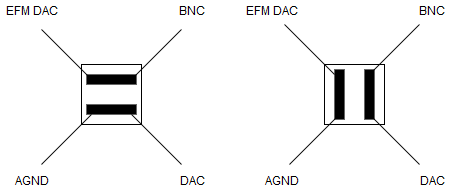
\includegraphics[scale = 0.6]{images/DAC_headers.png}
\caption{Left: Jumpers connecting \gls{mcu} \gls{dac} to \gls{bnc} and normal \gls{dac} to ground. Right: The opposite}
\label{fig:DAC headers}
\end{figure}

